\documentclass[a4paper]{article}
\usepackage[normalem]{ulem}
\usepackage{graphicx}
\usepackage[font=small,labelfont=bf]{caption}

% impostazioni generali
%Tutti gli usepackage vanno qui
\usepackage[table]{xcolor}
\usepackage{geometry}
\usepackage[italian]{babel}
\usepackage[utf8]{inputenc}
\usepackage{tabularx}
\usepackage{longtable}
\usepackage{hyperref}
\usepackage{enumitem}
\usepackage{array} 
\usepackage{booktabs}
\newcolumntype{M}[1]{>{\centering\arraybackslash}m{#1}}
\usepackage[toc]{appendix}
\usepackage{caption}

\hypersetup{
	colorlinks=true,
	linkcolor=blue,
	filecolor=magenta,
	urlcolor=blue,
}
% Numerazione figure
\let\counterwithout\relax
\let\counterwithin\relax
\usepackage{chngcntr}

% distanziare elenco delle figure e delle tabelle
\usepackage{tocbasic}
\DeclareTOCStyleEntry[numwidth=3.5em]{tocline}{figure}% for figure entries
\DeclareTOCStyleEntry[numwidth=3.5em]{tocline}{table}% for table entries


%\counterwithout{table}{section}
%\counterwithout{figure}{section}
\captionsetup[table]{font=small,skip=5pt} 

\usepackage[bottom]{footmisc}
\usepackage{fancyhdr}
\setcounter{secnumdepth}{4}
\usepackage{amsmath, amssymb}
\usepackage{array}
\usepackage{graphicx}

\usepackage{ifthen}

\usepackage{float}
\restylefloat{table}

\usepackage{layouts}
\usepackage{url}
\usepackage{comment}
\usepackage{eurosym}

\usepackage{lastpage}
\usepackage{layouts}
\usepackage{eurosym}

\geometry{a4paper,top=3cm,bottom=4cm,left=2.5cm,right=2.5cm}

%Comandi di impaginazione uguale per tutti i documenti
\pagestyle{fancy}
\lhead{
\includegraphics[scale=0.25]{template/images/logo-inline.png}}

%Titolo del documento

%\rfoot{\thepage}
\cfoot{Pagina \thepage\ di \pageref{LastPage}}
\setlength{\headheight}{35pt}
\setcounter{tocdepth}{5}
\setcounter{secnumdepth}{5}
\renewcommand{\footrulewidth}{0.4pt}

% multirow per tabelle
\usepackage{multirow}

% Permette tabelle su più pagine
%\usepackage{longtable}


%COMANDI TABELLE
\newcommand{\rowcolorhead}{\rowcolor[HTML]{731733}}
\newcommand{\captionline}{\rowcolor[HTML]{FFFFFF}} %comando per le caption delle tabelle
\newcommand{\cellcolorhead}{\cellcolor[HTML]{007c95}}
\newcommand{\hlinetable}{\arrayrulecolor[HTML]{007c95}\hline}

%intestazione
% check for missing commands
\newcommand{\headertitle}[1]{\textbf{\color{white}#1}} %titolo colonna
\definecolor{pari}{HTML}{dcbac2}
\definecolor{dispari}{HTML}{f5f5f5}

% comandi \textit{Glossario}
\newcommand{\glo}{$_{G}$}
\newcommand{\glosp}{$_{G}$ }

%comando signature
\newcommand\signature[2]{% Name; Department
\noindent\begin{minipage}{5cm}
    \noindent\vspace{3cm}\par
    \noindent\rule{5cm}{1pt}\par
    \noindent\textbf{#1}\par
    \noindent#2%
\end{minipage}}


%label custom
\makeatletter
\newcommand{\uclabel}[2]{%
	\protected@write \@auxout {}{\string \newlabel {#1}{{#2}{\thepage}{#2}{#1}{}} }%
	\hypertarget{#1}{#2}
}
\makeatother

%riportare pezzi di codice
\definecolor{codegray}{gray}{0.9}
\newcommand{\code}[1]{\colorbox{codegray}{\texttt{#1}}}

% dati relativi alla prima pagina
\makeindex
\begin{document}
\counterwithin{table}{section}

% Prima pagina
\thispagestyle{empty}
\renewcommand{\arraystretch}{1.3}


\begin{titlepage}
	\begin{center}
		
	
\includegraphics[scale = 0.6]{template/images/logo-circle.png}
	\\[0.8cm]
	\href{mailto:6bitbusters@gmail.com}		      	
	{\large{\textit{6bitbusters@gmail.com} } }\\[0.8cm]
	
	\Huge \textbf{Norme di progetto} \\[0.5cm]

	% Informazioni sul documento
	\large \textbf{Informazioni sul documento} \\
	\rule{0.6\textwidth}{0.4pt}
	\\[0.5cm]
	\begin{tabular}{r|l}
		\textbf{Versione} & 1.0.0\\
		\textbf{Stato} & Approvato\\
		\textbf{Uso} & Interno\\                         
		\textbf{Approvazione} & Soranzo Andrea\\                      
		\textbf{Verifica} & Pincin Matteo\\ & Diviesti Filippo\\ & Bergamin Elia\\ & Djossa Edgar\\                        
		\textbf{Redazione} & Djossa Edgar \\ & Pincin Matteo \\ & Soranzo Andrea\\ & Chilese Elena \\ & Bergamin Elia\\
		\textbf{Distribuzione} & \textit{Six Bit Busters} \\ & Prof. Vardanega Tullio \\ & Prof. Cardin Riccardo
	\end{tabular}	
	\\[0.8cm]

 % Descrizione
	\large \textbf{Descrizione} \\
	Questo documento contiene le norme di progetto seguite dal gruppo \textit{Six Bit Busters}.
	
	
	
	\end{center}
\end{titlepage}


% Diario delle modifiche

\section*{Registro delle modifiche}

\newcommand{\changelogTable}[1]{

\renewcommand{\arraystretch}{1.5}
\rowcolors{2}{pari}{dispari}
\begin{longtable}{ %0.87
		>{\centering}M{0.10\textwidth} 
		>{\centering}M{0.11\textwidth}
		>{\centering}M{0.19\textwidth}
		>{\centering}M{0.28\textwidth} 
		>{\centering\arraybackslash}M{0.19\textwidth} 
		 }
	\rowcolorhead
	\headertitle{Versione} &
	\centering \headertitle{Data} &	
	\headertitle{Autore} &
	\headertitle{Descrizione} & 
	\headertitle{Verificatore} 
	\endfirsthead	
	\endhead
	
	#1

\end{longtable}
\vspace{-2em}

}


\changelogTable{
1.0.0& xxx & xxx & - &  Approvazione documento\tabularnewline
0.1.0& xxx & xxx & - &  Verifica documento\tabularnewline
0.0.3& xxx & xxx & - &  Stesura pro e contro\tabularnewline
	0.0.2& xxx & xxx & - &  Stesura introduzione\tabularnewline
	0.0.1 & 17-10-2024 & Chilese Elena & - &  Creazione struttura e template documento \\
}
\pagebreak

% Indice
{
    \hypersetup{linkcolor=black}
    \tableofcontents
}
\pagebreak

\hypersetup{colorlinks=false, linkcolor=black}
\listoffigures
\hypersetup{colorlinks=true, linkcolor=blue}

% Contenuto
\section{Introduzione}
    \subsection{Scopo del documento}
    Questo documento ha lo scopo di definire le norme e le linee guida operative per il team \textit{Six Bit Busters} nello sviluppo del progetto \textit{3Dataviz}.\\ 
    In particolare, esso descrive i processi di lavoro, le modalità di collaborazione, gli standard di codifica e le pratiche di gestione della qualità che il team seguirà per garantire coerenza, efficienza e qualità durante il ciclo di vita del prodotto. 
    Lo scopo è quello di fornire una struttura comrune e procedure chiare, per facilitare il lavoro di squadra, garantendo che tutti i membri operino in linea con gli obiettivi e le specifiche concordate.
ddfflsdsddddddddgfglldddddsdsdgggdadfffffffff
    \subsection{Scopo del prodotto}
    \textit{3Dataviz} è un prodotto ideato dall'azienda \textit{Sanmarco Informatica S.p.A.} per semplificare e rendere più accessibile la visualizzazione dei dati.\\
    Il progetto si basa sul concetto di data visualization, che consiste nel trasformare i dati in grafici e rappresentazioni visive, sfruttando la capacità del cervello umano di elaborare rapidamente le immagini. 
    Questo approccio facilita il processo decisionale e migliora la comprensione delle informazioni.\\
    L’obiettivo principale è lo sviluppo di un’interfaccia web che trasforma dati provenienti da diverse fonti (come database e REST API) in grafici 3D interattivi e navigabili. 
    Inoltre, i dati potranno essere consultati anche in formato tabellare, offrendo una visione alternativa ma altrettanto utile.  

    \subsection{Glossario}
    Per chiarire i termini tecnici o ambigui si utilizza un glossario disponibile nel file \textit{Glossario}.\\
    Tutti i termini che richiedono spiegazioni sono indicati con il pedice “g”. \\
    Questa convenzione consente un rapido collegamento tra il testo principale e la relativa spiegazione dettagliata nel glossario, garantendo coerenza e chiarezza nella comunicazione.

    \subsection{Riferimenti}
        \subsubsection{Riferimenti normativi}
        \begin{itemize}
            \item Capitolato d'appalto C5 \textit{Sanmarco Informatica S.p.A.} - 3Dataviz : \\ \url{https://www.math.unipd.it/~tullio/IS-1/2024/Progetto/C5.pdf}
            \item Materiale didattico - Corso Ingegneria del software 2024/2025 - Regolamento del Progetto Didattico: \\ \url{https://www.math.unipd.it/~tullio/IS-1/2024/Dispense/PD1.pdf}
        \end{itemize}
        \subsubsection{Riferimenti informativi}
        \begin{itemize}
            \item Materiale didattico - Corso Ingegneria del software 2024/2025 - Processi di ciclo di vita: \\ \url{https://www.math.unipd.it/~tullio/IS-1/2024/Dispense/T02.pdf}
            \item Materiale didattico - Corso Ingegneria del software 2024/2025 - Il ciclo di vita del SW: \\ \url{https://www.math.unipd.it/~tullio/IS-1/2024/Dispense/T03.pdf}
            \item Materiale didattico - Corso Ingegneria del software 2024/2025 - Gestione di progetto: \\ \url{https://www.math.unipd.it/~tullio/IS-1/2024/Dispense/T04.pdf}
            \item Materiale didattico - Corso Ingegneria del software 2024/2025 - Verifica e validazione: analisi dinamica: \\ \url{https://www.math.unipd.it/~tullio/IS-1/2024/Dispense/T11.pdf}
            \item Riferimento per alcune metriche di processo: \\ \url{https://it.wikipedia.org/wiki/Metriche_di_progetto}
            \item Indice Gulpease: \\ \url{https://it.wikipedia.org/wiki/Indice_Gulpease}
            \item Requirements Stability Index (RSI): \\ \url{https://shiyamtj.wordpress.com/2018/09/26/requirement-stability-index/}
        
        \end{itemize}

\pagebreak

\newcounter{UC}
\newcounter{SUC}
\newcounter{SSUC}

\newcommand{\resetCounter}[1]{%
    \setcounter{#1}{0}
}

\newcommand{\UseCase}[1]{%
    \refstepcounter{UC}
    \resetCounter{SUC}
    \resetCounter{SSUC}
    \subsection{UC\arabic{UC} - #1}\label{UC:\arabic{UC}}
}

\newcommand{\SubUseCase}[1]{%
    \stepcounter{SUC}
    \resetCounter{SSUC}
    \subsubsection{UC\arabic{UC}.\arabic{SUC} - #1}\label{UC:\arabic{UC}.\arabic{SUC}}
}

\newcommand{\SubSubUseCase}[1]{%
    \stepcounter{SSUC}  
    \paragraph{UC\arabic{UC}.\arabic{SUC}.\arabic{SSUC} - #1}
}

% COME UTILIZZARE I CASI D`USO:
% i comandi di use case vanno utilizzati al posto di subsection, subsubsection e paragraph

% \UseCase => rappresenta lo use case principale (UC1,UC2,UC3)
% \SubUseCase => rappresenta il primo sotto livello dello use case principale (UC1.1,UC2.1,UC3.3)
% \SubSubUseCase => rappresenta il secondo sotto livello dello lo use case principale (UC1.1.1,UC2.1.2,UC3.3.1)

\newcommand{\UCdsc}[5]{
    \begin{itemize}
        \item \textbf{Attore primario:}
         #1
        \item \textbf{Descrizione:} 
         #2
        \item \textbf{Precondizioni:}
         #3
        \item \textbf{Postcondizioni:}
        #4
        \item \textbf{Scenario principale:} 
        #5
    \end{itemize}
}


\GetTitleStringSetup{expand}
\section{Casi d'uso}
% \subsection{Attore}
% Poiché per lo svolgimento del progetto non è necessario gestire permessi differenti per l'accesso alle funzionalità, l'attore che interagisce con il nostro software è unico, denominato "Utente".\\
% \textbf{Utente:} soggetto che utilizza la web application, sfruttandone le funzionalità.

% UC1 - UC11

\UseCase{Visualizza lista dataset}
    \begin{figure}[h!]
        \centering
        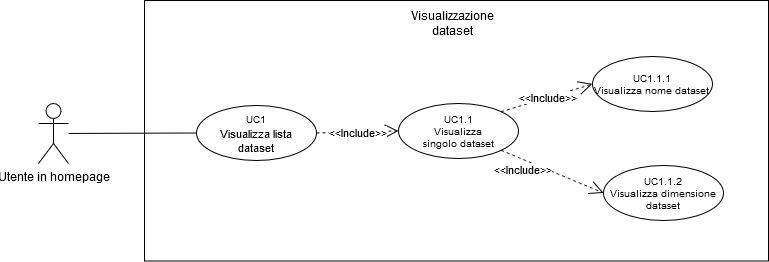
\includegraphics[scale=0.55]{template/images/UC1.png}
        \caption{\nameref*{UC:\arabic{UC}}}
    \end{figure}
    \UCdsc
    { % ATTORE
        \begin{itemize}
            \item Utente in homepage.
        \end{itemize}
    }
    { % DESCRIZIONE
        \begin{itemize}
            \item All'avvio del sistema l'utente visualizza la lista completa dei dataset proposti.
        \end{itemize}
    }
    { % PRECONDIZIONI
        \begin{itemize}
            \item L'utente ha accesso all'applicazione.
        \end{itemize}
    }
    { % POSTCONDIZIONI
        \begin{itemize}
            \item L'utente vede la lista dei dataset disponibili.
        \end{itemize}
    }
    { % SCENARIO PRIMARIO
        \begin{itemize}
            \item L'utente avvia il sistema.
        \end{itemize}
    }


    \newpage

    \SubUseCase{Visualizza singolo dataset}
    \UCdsc
    { % ATTORE
        \begin{itemize}
            \item Utente in homepage.
        \end{itemize}
    }
    { % DESCRIZIONE
        \begin{itemize}
            \item Visualizzazione dei singoli dataset di cui la lista è composta.
        \end{itemize}
    }
    { % PRECONDIZIONI
        \begin{itemize}
            \item La lista dei dataset è visibile.
        \end{itemize}
    }
    { % POSTCONDIZIONI
        \begin{itemize}
            \item Il dataset è visibile nella lista dei dataset.
        \end{itemize}
    }
    { % SCENARIO PRIMARIO
        \begin{itemize}
            \item Nessuna azione richiesta.
        \end{itemize}
    }

    \SubSubUseCase{Visualizza nome dataset}
    \UCdsc
    { % ATTORE
        \begin{itemize}
            \item Utente in homepage.
        \end{itemize}
    }
    { % DESCRIZIONE
        \begin{itemize}
            \item Visualizzazione del nome del dataset. Quest'ultimo è considerato come un identificativo che permette di distinguere i diversi dataset.
        \end{itemize}
    }
    { % PRECONDIZIONI
        \begin{itemize}
            \item Il dataset è presente della lista dei dataset.
        \end{itemize}
    }
    { % POSTCONDIZIONI
        \begin{itemize}
            \item Il nome del dataset è visibile.
        \end{itemize}
    }
    { % SCENARIO PRIMARIO
        \begin{itemize}
            \item Nessuna azione richiesta.
        \end{itemize}
    }


    \SubSubUseCase{Visualizza dimensione dataset}
    \UCdsc
    { % ATTORE
        \begin{itemize}
            \item Utente in homepage.
        \end{itemize}
    }
    { % DESCRIZIONE
        \begin{itemize}
            \item Visualizzazione della dimensione del dataset.
        \end{itemize}
    }
    { % PRECONDIZIONI
        \begin{itemize}
            \item Il dataset è presente della lista dei dataset.
        \end{itemize}
    }
    { % POSTCONDIZIONI
        \begin{itemize}
            \item La dimensione del dataset è visibile.
        \end{itemize}
    }
    { % SCENARIO PRIMARIO
        \begin{itemize}
            \item Nessuna azione richiesta.
        \end{itemize}
    }


\UseCase{Visualizza dettaglio dataset}
    \begin{figure}[h!]
        \centering
        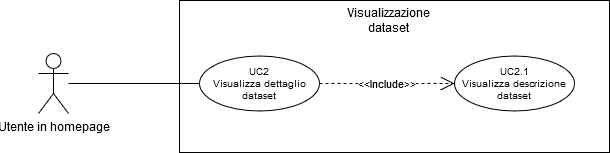
\includegraphics[scale=0.6]{template/images/UC2.png}
        \caption{\nameref*{UC:\arabic{UC}}}
    \end{figure}
    \UCdsc
    { % ATTORE
        \begin{itemize}
            \item Utente in homepage.
        \end{itemize}
    }
    { % DESCRIZIONE
        \begin{itemize}
            \item L'utente può visualizzare i dettagli di un dataset, ossia le sue informazioni aggiuntive.
        \end{itemize}
    }
    { % PRECONDIZIONI
        \begin{itemize}
            \item Il dataset deve essere un dataset proposto.
        \end{itemize}
    }
    { % POSTCONDIZIONI
        \begin{itemize}
            \item I dettagli del dataset sono visibili.
        \end{itemize}
    }
    { % SCENARIO PRIMARIO
        \begin{itemize}
            \item L'utente interagisce con il sistema espandendo la vista del singolo dataset.
        \end{itemize}
    }
    

    \SubUseCase{Visualizza descrizione dataset}
    \UCdsc
    { % ATTORE
        \begin{itemize}
            \item Utente in homepage.
        \end{itemize}
    }
    { % DESCRIZIONE
        \begin{itemize}
            \item Visualizzazione della descrizione del dataset.
        \end{itemize}
    }
    { % PRECONDIZIONI
        \begin{itemize}
            \item I dettagli del dataset sono visibili.
        \end{itemize}
    }
    { % POSTCONDIZIONI
        \begin{itemize}
            \item La descrizione del dataset è visibile.
        \end{itemize}
    }
    { % SCENARIO PRIMARIO
        \begin{itemize}
            \item Nessuna azione richiesta.
        \end{itemize}
    }



\UseCase{Carica dataset}
\begin{figure}[h!]
    \centering
    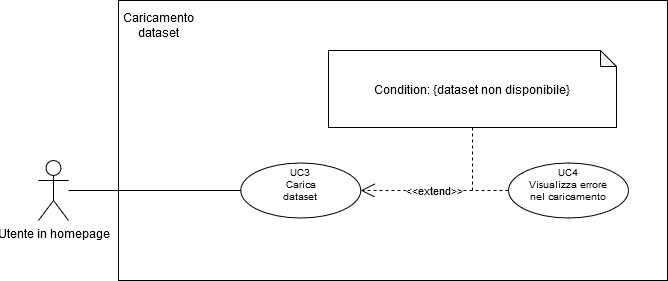
\includegraphics[scale=0.6]{template/images/UC3.png}
    \caption{\nameref*{UC:\arabic{UC}}}
\end{figure}
    \UCdsc
    { % ATTORE
        \begin{itemize}
            \item Utente in homepage.
        \end{itemize}
    }
    { % DESCRIZIONE
        \begin{itemize}
            \item L'utente decide il dataset che vuole visualizzare andando quindi a caricare tutti i dati e i valori nel sistema.
        \end{itemize}
    }
    { % PRECONDIZIONI
        \begin{itemize}
            \item La lista dei dataset disponibili è visibile.
        \end{itemize}
    }
    { % POSTCONDIZIONI
        \begin{itemize}
            \item Il dataset viene caricato nel sistema;
            \item L'utente entra nell'ambiente 3D.
        \end{itemize}
    }
    { % SCENARIO PRIMARIO
        \begin{itemize}
            \item L'utente seleziona un dataset tra quelli proposti nella lista.
        \end{itemize}
        % ESTENSIONE
        \item \textbf{Estensione:} \begin{itemize}
            \item UC4 - Visualizza errore nel caricamento.
        \end{itemize}
    }


\newpage

\UseCase{Visualizza errore nel caricamento}
    \UCdsc
    { % ATTORE
        \begin{itemize}
            \item Utente in homepage.
        \end{itemize}
    }
    { % DESCRIZIONE
        \begin{itemize}
            \item Visualizzazione di un messaggio di errore "Dataset non disponibile" con una motivazione a seguire.
                    Il caricamento potrebbe fallire perchè il dataset selezionato potrebbe essere
                    non disponibile in quel momento o ci potrebbe essere un errore di connessione.
        \end{itemize}
    }
    { % PRECONDIZIONI
        \begin{itemize}
            \item L'utente ha selezionato un dataset;
            \item Il dataset selezionato non è disponibile.
        \end{itemize}
    }
    { % POSTCONDIZIONI
        \begin{itemize}
            \item Il dataset non viene caricato nel sistema;
            \item L'utente torna alla vista della lista di dataset.
        \end{itemize}
    }
    { % SCENARIO PRIMARIO
        \begin{itemize}
            \item Nessuna azione richiesta.
        \end{itemize}
    }



\UseCase{Visualizza dataset in forma tabellare}
\begin{figure}[h!]
    \centering
    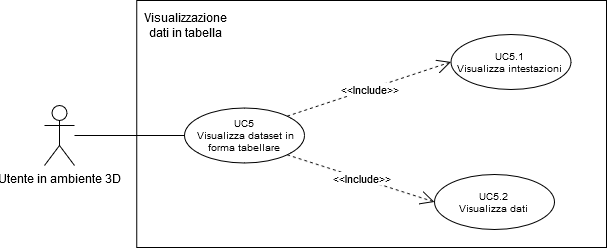
\includegraphics[scale=0.7]{template/images/UC5.png}
    \caption{\nameref*{UC:\arabic{UC}}}
\end{figure}
\UCdsc
    { % ATTORE
        \begin{itemize}
            \item Utente in ambiente 3D.
        \end{itemize}
    }
    { % DESCRIZIONE
        \begin{itemize}
            \item Visualizzazione del dataset caricato in forma tabellare.
        \end{itemize}
    }
    { % PRECONDIZIONI
        \begin{itemize}
            \item L'utente è all'interno dell'ambiente 3D;
            \item Il caricamento del dataset è terminato.
        \end{itemize}
    }
    { % POSTCONDIZIONI
        \begin{itemize}
            \item La tabella contenente i dati del dataset è visibile con i rispettivi valori.
        \end{itemize}
    }
    { % SCENARIO PRIMARIO
        \begin{itemize}
            \item Nessuna azione richiesta.
        \end{itemize}
    }


\SubUseCase{Visualizza intestazioni}
\UCdsc
    { % ATTORE
        \begin{itemize}
            \item Utente in ambiente 3D.
        \end{itemize}
    }
    { % DESCRIZIONE
        \begin{itemize}
            \item Visualizzazione delle intestazioni della tabella contenente tutti i valori del dataset selezionato.
        \end{itemize}
    }
    { % PRECONDIZIONI
        \begin{itemize}
            \item La tabella è visibile.
        \end{itemize}
    }
    { % POSTCONDIZIONI
        \begin{itemize}
            \item Le intestazioni della tabella sono visibili.
        \end{itemize}
    }
    { % SCENARIO PRIMARIO
        \begin{itemize}
            \item Nessuna azione richiesta.
        \end{itemize}
    }

\SubUseCase{Visualizza dati}
\UCdsc
    { % ATTORE
        \begin{itemize}
            \item Utente in ambiente 3D.
        \end{itemize}
    }
    { % DESCRIZIONE
        \begin{itemize}
            \item Visualizzazione di tutti i valori del dataset selezionato attraverso le celle della tabella.
        \end{itemize}
    }
    { % PRECONDIZIONI
        \begin{itemize}
            \item La tabella è visibile.
        \end{itemize}
    }
    { % POSTCONDIZIONI
        \begin{itemize}
            \item I valori del dataset selezionato vengono visualizzati nella tabella.
        \end{itemize}
    }
    { % SCENARIO PRIMARIO
        \begin{itemize}
            \item Nessuna azione richiesta.
        \end{itemize}
    }

\UseCase{Visualizza dataset tramite grafico 3D}
\begin{figure}[h!]
    \centering
    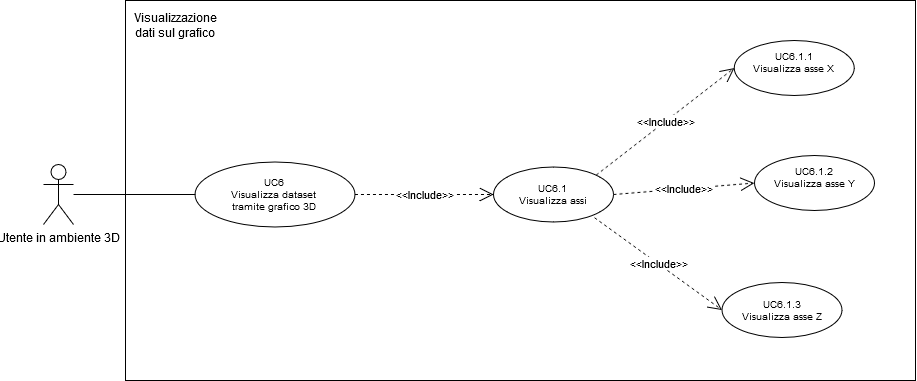
\includegraphics[scale=0.45]{template/images/UC6.png}
    \caption{\nameref*{UC:\arabic{UC}}}
\end{figure}
\UCdsc
    { % ATTORE
        \begin{itemize}
            \item Utente in ambiente 3D.
        \end{itemize}
    }
    { % DESCRIZIONE
        \begin{itemize}
            \item Visualizzazione del dataset caricato sotto forma di grafico 3D a barre verticali.
        \end{itemize}
    }
    { % PRECONDIZIONI
        \begin{itemize}
            \item L'utente è all'interno dell'ambiente 3D;
            \item Il caricamento del dataset è terminato.
        \end{itemize}
    }
    { % POSTCONDIZIONI
        \begin{itemize}
            \item Il grafico 3D è visibile.
        \end{itemize}
    }
    { % SCENARIO PRIMARIO
        \begin{itemize}
            \item Nessuna azione richiesta.
        \end{itemize}
    }


\SubUseCase{Visualizza assi}
\UCdsc
    { % ATTORE
        \begin{itemize}
            \item Utente in ambiente 3D.
        \end{itemize}
    }
    { % DESCRIZIONE
        \begin{itemize}
            \item Visualizzazione degli assi X, Y e Z del grafico 3D.
        \end{itemize}
    }
    { % PRECONDIZIONI
        \begin{itemize}
            \item Il grafico 3D è visibile.
        \end{itemize}
    }
    { % POSTCONDIZIONI
        \begin{itemize}
            \item Gli assi del grafico 3D sono visibili.
        \end{itemize}
    }
    { % SCENARIO PRIMARIO
        \begin{itemize}
            \item Nessuna azione richiesta.
        \end{itemize}
    }

\SubSubUseCase{Visualizza asse X}
\UCdsc
    { % ATTORE
        \begin{itemize}
            \item Utente in ambiente 3D.
        \end{itemize}
    }
    { % DESCRIZIONE
        \begin{itemize}
            \item Visualizzazione dell'asse X del grafico 3D con le sue eventuali etichette.
        \end{itemize}
    }
    { % PRECONDIZIONI
        \begin{itemize}
            \item Il grafico 3D è visibile.
        \end{itemize}
    }
    { % POSTCONDIZIONI
        \begin{itemize}
            \item L'asse X del grafico 3D è visibile;
            \item Le etichette dell'asse X del grafico 3D sono visibili.
        \end{itemize}
    }
    { % SCENARIO PRIMARIO
        \begin{itemize}
            \item Nessuna azione richiesta.
        \end{itemize}
    }

\SubSubUseCase{Visualizza asse Y}
\UCdsc
    { % ATTORE
        \begin{itemize}
            \item Utente in ambiente 3D.
        \end{itemize}
    }
    { % DESCRIZIONE
        \begin{itemize}
            \item Visualizzazione dell'asse Y del grafico 3D con le sue eventuali etichette.
        \end{itemize}
    }
    { % PRECONDIZIONI
        \begin{itemize}
            \item Il grafico 3D è visibile.
        \end{itemize}
    }
    { % POSTCONDIZIONI
        \begin{itemize}
            \item L'asse Y del grafico 3D è visibile;
            \item Le etichette dell'asse Y del grafico 3D sono visibili.
        \end{itemize}
    }
    { % SCENARIO PRIMARIO
        \begin{itemize}
            \item Nessuna azione richiesta.
        \end{itemize}
    }

\SubSubUseCase{Visualizza asse Z}
\UCdsc
    { % ATTORE
        \begin{itemize}
            \item Utente in ambiente 3D.
        \end{itemize}
    }
    { % DESCRIZIONE
        \begin{itemize}
            \item Visualizzazione dell'asse Z del grafico 3D con le sue eventuali etichette.
        \end{itemize}
    }
    { % PRECONDIZIONI
        \begin{itemize}
            \item Il grafico 3D è visibile.
        \end{itemize}
    }
    { % POSTCONDIZIONI
        \begin{itemize}
            \item L'asse Z del grafico 3D è visibile;
            \item Le etichette dell'asse Z del grafico 3D sono visibili.
        \end{itemize}
    }
    { % SCENARIO PRIMARIO
        \begin{itemize}
            \item Nessuna azione richiesta.
        \end{itemize}
    }


\UseCase{Spostamento orizzontale della telecamera}
    \begin{figure}[h!]
        \centering
        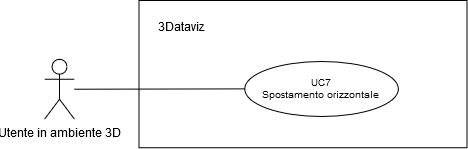
\includegraphics[scale=0.65]{template/images/UC7.png}
        \caption{\nameref*{UC:\arabic{UC}}}
    \end{figure}
    \UCdsc
        { % ATTORE
            \begin{itemize}
                \item Utente in ambiente 3D.
            \end{itemize}
        }
        { % DESCRIZIONE
            \begin{itemize}
                \item Spostare la telecamera orizzontalmente significa far scorrere la vista a destra o a sinistra, mantenendo la stessa inclinazione.
            \end{itemize}
        }
        { % PRECONDIZIONI
            \begin{itemize}
                \item Le azioni di movimento devono essere valide. Un'azione di movimento è valida se non va oltre il margine destro o sinistro di un'area predefinita dal sistema;
                \item La telecamera si trova in una posizione arbitraria nello spazio.
            \end{itemize}
        }
        { % POSTCONDIZIONI
            \begin{itemize}
                \item  La telecamera si trova in una posizione orizzontale scelta dall'utente, diversa da quella iniziale.
            \end{itemize}
        }
        { % SCENARIO PRIMARIO
            \begin{itemize}
                \item L'utente interagisce con il sistema per compiere un'azione di movimento di spostamento orizzontale.
            \end{itemize}
        }

\UseCase{Spostamento verticale della telecamera}
    \begin{figure}[h!]
        \centering
        
\includegraphics[scale=0.65]{template/images/UC8.png}
        \caption{\nameref*{UC:\arabic{UC}}}
    \end{figure}
    \UCdsc
        { % ATTORE
            \begin{itemize}
                \item Utente in ambiente 3D.
            \end{itemize}
        }
        { % DESCRIZIONE
            \begin{itemize}
                \item Spostare la telecamera verticale significa far scorrere la vista in alto o in basso, mantenendo la stessa inclinazione.
            \end{itemize}
        }
        { % PRECONDIZIONI
            \begin{itemize}
                \item Le azioni di movimento devono essere valide. Un'azione di movimento è valida se non va oltre il margine superiore o inferiore di un'area predefinita dal sistema;
                \item La telecamera si trova in una posizione arbitraria nello spazio.
            \end{itemize}
        }
        { % POSTCONDIZIONI
            \begin{itemize}
                \item La telecamera si trova in una posizione verticale scelta dall'utente, diversa da quella iniziale.
            \end{itemize}
        }
        { % SCENARIO PRIMARIO
            \begin{itemize}
                \item L'utente interagisce con il sistema per compiere un'azione di movimento di spostamento verticale.
            \end{itemize}
        }

\UseCase{Ruota grafico attorno asse X}
\begin{figure}[h!]
    \centering
    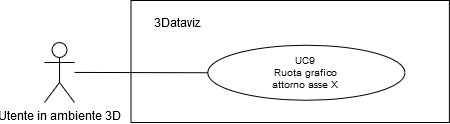
\includegraphics[scale=0.65]{template/images/UC9.png}
    \caption{\nameref*{UC:\arabic{UC}}}
\end{figure}
\UCdsc
{ % ATTORE
    \begin{itemize}
        \item Utente in ambiente 3D.
    \end{itemize}
}
{ % DESCRIZIONE
    \begin{itemize}
        \item L'attore compie un'azione di rotazione del grafico attorno all'asse X.
    \end{itemize}
}
{ % PRECONDIZIONI
    \begin{itemize}
        \item Il grafico è visibile;
        \item Il grafico ha una rotazione arbitraria.
    \end{itemize}
}
{ % POSTCONDIZIONI
    \begin{itemize}
        \item Il grafico ha una rotazione scelta dall'utente, diversa rispetto a quella iniziale.
    \end{itemize}
}
{ % SCENARIO PRIMARIO
    \begin{itemize}
        \item L'utente interagisce con il sistema per compiere un'azione di rotazione del grafico attorno all'asse X.
    \end{itemize}
}

\UseCase{Ruota grafico attorno asse Y}
\begin{figure}[h!]
    \centering
    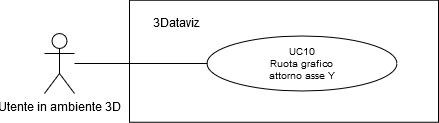
\includegraphics[scale=0.65]{template/images/UC10.png}
    \caption{\nameref*{UC:\arabic{UC}}}
\end{figure}
\UCdsc
{ % ATTORE
    \begin{itemize}
        \item Utente in ambiente 3D.
    \end{itemize}
}
{ % DESCRIZIONE
    \begin{itemize}
        \item L'attore compie un'azione di rotazione del grafico attorno all'asse Y.
    \end{itemize}
}
{ % PRECONDIZIONI
    \begin{itemize}
        \item Il grafico è visibile;
        \item Il grafico ha una rotazione arbitraria.
    \end{itemize}
}
{ % POSTCONDIZIONI
    \begin{itemize}
        \item Il grafico ha una rotazione scelta dall'utente, diversa rispetto a quella iniziale.
    \end{itemize}
}
{ % SCENARIO PRIMARIO
    \begin{itemize}
        \item L'utente interagisce con il sistema per compiere un'azione di rotazione del grafico attorno all'asse Y.
    \end{itemize}
}

\UseCase{Ruota grafico attorno asse Z}
\begin{figure}[h!]
    \centering
    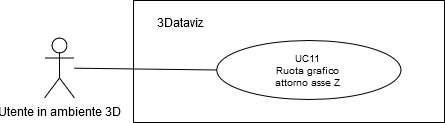
\includegraphics[scale=0.65]{template/images/UC11.png}
    \caption{\nameref*{UC:\arabic{UC}}}
\end{figure}
\UCdsc
{ % ATTORE
    \begin{itemize}
        \item Utente in ambiente 3D.
    \end{itemize}
}
{ % DESCRIZIONE
    \begin{itemize}
        \item L'attore compie un'azione di rotazione del grafico attorno all'asse Z.
    \end{itemize}
}
{ % PRECONDIZIONI
    \begin{itemize}
        \item Il grafico è visibile;
        \item Il grafico ha una rotazione arbitraria.
    \end{itemize}
}
{ % POSTCONDIZIONI
    \begin{itemize}
        \item Il grafico ha una rotazione scelta dall'utente, diversa rispetto a quella iniziale.
    \end{itemize}
}
{ % SCENARIO PRIMARIO
    \begin{itemize}
        \item L'utente interagisce con il sistema per compiere un'azione di rotazione del grafico attorno all'asse Z.
    \end{itemize}
}
    

%UC12 - UC19
\UseCase{Zoom della vista}
\begin{figure}[h!]\centering
    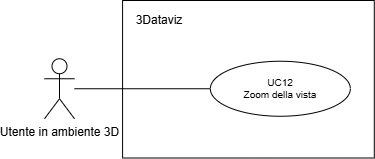
\includegraphics[scale=0.6]{template/images/UC12.png}
    \caption{\nameref*{UC:\arabic{UC}}}
\end{figure}
\UCdsc
{ % ATTORE
    \begin{itemize}
        \item Utente in ambiente 3D.
    \end{itemize}
}
{ % DESCRIZIONE
    \begin{itemize}
        \item Lo zoom consente all'utente di interagire con l'ambiente effettuando spostamenti lungo l'asse della profondità.
    \end{itemize}
}
{ % PRECONDIZIONI
    \begin{itemize}
        \item L'azione di zoom deve essere valida. Un'azione di zoom è valida se non va al di fuori di un'area predefinita dal sistema;
        \item La telecamera si trova in una posizione arbitraria nello spazio.
    \end{itemize}
}
{ % POSTCONDIZIONI
    \begin{itemize}
        \item La telecamera si trova in una posizione diversa da quella iniziale in termini di profondità.
    \end{itemize}
}
{ % SCENARIO PRIMARIO
    \begin{itemize}
        \item L'utente interagisce con il sistema per compiere un'azione di zoom.
    \end{itemize}
} 


\UseCase{Riposiziona telecamera alla posizione d’origine}
\begin{figure}[H]\centering
    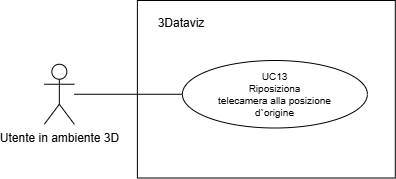
\includegraphics[scale=0.7]{template/images/UC13.png}
    \caption{\nameref*{UC:\arabic{UC}}}
\end{figure}
\UCdsc
{ % ATTORE
    \begin{itemize}
        \item Utente in ambiente 3D.
    \end{itemize}
}
{ % DESCRIZIONE
    \begin{itemize}
        \item Prevede il riposizionamento della telecamera nella posizione iniziale, corrispondente a quella definita durante la creazione dell'ambiente 3D.
    \end{itemize}
}
{ % PRECONDIZIONI
    \begin{itemize}
        \item La telecamera si trova in una posizione arbitraria nello spazio.
    \end{itemize}
}
{ % POSTCONDIZIONI
    \begin{itemize}
        \item La telecamera si trova nella posizione predefinita iniziale.
    \end{itemize}
}
{ % SCENARIO PRIMARIO
    \begin{itemize}
        \item L'utente seleziona il comando per riposizionare la telecamera.
    \end{itemize}
} 



\UseCase{Vista di una barra in primo piano}
\begin{figure}[h!]\centering
    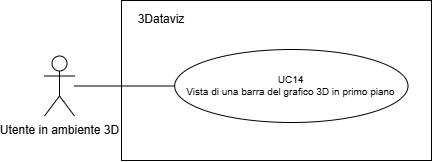
\includegraphics[scale=0.7]{template/images/UC14.png}
    \caption{\nameref*{UC:\arabic{UC}}}
\end{figure}
\UCdsc
{ % ATTORE
    \begin{itemize}
        \item Utente in ambiente 3D.
    \end{itemize}
}
{ % DESCRIZIONE
    \begin{itemize}
        \item La visualizzazione di una barra in primo piano consiste nel posizionare la telecamera in modo da massimizzare la visibilità di una specifica barra all'interno della scena, garantendo che sia sempre presente nel campo visivo dell'utente.
    \end{itemize}
}
{ % PRECONDIZIONI
    \begin{itemize}
        \item Il grafico è visibile;
        \item La telecamera si trova in una posizione arbitraria;
        \item L'utente ha selezionato un valore del dataset associato ad una barra.
    \end{itemize}
}
{ % POSTCONDIZIONI
    \begin{itemize}
        \item La telecamera è stata riposizionata per mettere in primo piano la barra selezionata.
    \end{itemize}
}
{ % SCENARIO PRIMARIO
    \begin{itemize}
        \item L'utente seleziona un valore del dataset che corrisponde ad una barra sul grafico 3D.
    \end{itemize}
}


\UseCase{Visualizza dettagli di una barra del grafico 3D}
\begin{figure}[H]\centering
    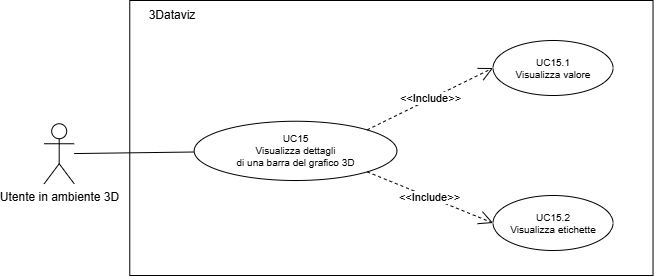
\includegraphics[scale=0.7]{template/images/UC15.png}
    \caption{\nameref*{UC:\arabic{UC}}}
\end{figure}
\UCdsc
{ % ATTORE
    \begin{itemize}
        \item Utente in ambiente 3D.
    \end{itemize}
}
{ % DESCRIZIONE
    \begin{itemize}
        \item L'utente può visualizzare i dettagli di una barra del grafico, come il valore e le etichette a lei associate.
    \end{itemize}
}
{ % PRECONDIZIONI
    \begin{itemize}
        \item Il grafico è visibile;
        \item La barra è visibile.
    \end{itemize}
}
{ % POSTCONDIZIONI
    \begin{itemize}
        \item I dettagli della barra sono visibili.
    \end{itemize}
}
{ % SCENARIO PRIMARIO
    \begin{itemize}
        \item L'utente interagisce con la barra tramite hover o selezione.
    \end{itemize}
}

\SubUseCase{Visualizza valore}
\UCdsc
{ % ATTORE
    \begin{itemize}
        \item Utente in ambiente 3D.
    \end{itemize}
}
{ % DESCRIZIONE
    \begin{itemize}
        \item Visualizzazione del valore della barra.
    \end{itemize}
}
{ % PRECONDIZIONI
    \begin{itemize}
        \item I dettagli della barra sono visibili.
    \end{itemize}
}
{ % POSTCONDIZIONI
    \begin{itemize}
        \item Il valore della barra è visibile.
    \end{itemize}
}
{ % SCENARIO PRIMARIO
    \begin{itemize}
        \item Nessuna azione richiesta. 
    \end{itemize}
}

\SubUseCase{Visualizza etichette}
\UCdsc
{ % ATTORE
    \begin{itemize}
        \item Utente in ambiente 3D.
    \end{itemize}
}
{ % DESCRIZIONE
    \begin{itemize}
        \item Visualizzazione delle etichette associate alla barra.
    \end{itemize}
}
{ % PRECONDIZIONI
    \begin{itemize}
        \item I dettagli della barra sono visibili.
    \end{itemize}
}
{ % POSTCONDIZIONI
    \begin{itemize}
        \item Le etichette della barra sono visibili.
    \end{itemize}
}
{ % SCENARIO PRIMARIO
    \begin{itemize}
        \item Nessuna azione richiesta. 
    \end{itemize}
}

\UseCase{Filtra un numero N di valori}
\begin{figure}[h!]\centering
    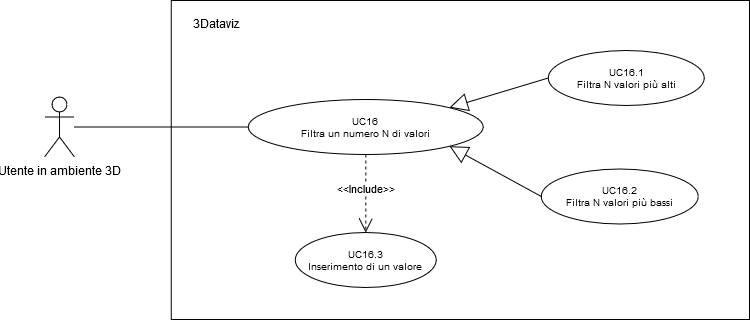
\includegraphics[scale=0.6]{template/images/UC16.png}
    \caption{\nameref*{UC:\arabic{UC}}}
\end{figure}
\UCdsc
{ % ATTORE
    \begin{itemize}
        \item Utente in ambiente 3D.
    \end{itemize}
}
{ % DESCRIZIONE
    \begin{itemize}
        \item Questo filtro consente all'utente di visualizzare solo le barre che corrispondono ai primi N valori più alti o più bassi. 
        N rappresenta il numero massimo di valori da considerare.
    \end{itemize}
}
{ % PRECONDIZIONI
    \begin{itemize}
        \item Il grafico è visibile.
    \end{itemize}
}
{ % POSTCONDIZIONI
    \begin{itemize}
        \item È stato applicato il filtro per visualizzare solo le prime N barre più alte o più basse.
    \end{itemize}
}
{ % SCENARIO PRIMARIO
    \begin{itemize}
        \item L'utente inserisce un numero N;
        \item L'utente seleziona il filtro;
        \item Il sistema aggiorna la visualizzazione del grafico, mostrando solo le barre che rientrano tra le prime N più alte o più basse.
    \end{itemize}
        % GENERALIZZAZIONI
        \item \textbf{Generalizzazioni:} \begin{itemize}
            \item UC16.1 - Filtra N valori più alti;
            \item UC16.2 - Filtra N valori più bassi.
        \end{itemize}
}

\SubUseCase{Filtra N valori più alti}
\UCdsc
{ % ATTORE
    \begin{itemize}
        \item Utente in ambiente 3D.
    \end{itemize}
}
{ % DESCRIZIONE
    \begin{itemize}
        \item L'utente decide di evidenziare gli N valori più alti, rendendo visibili le barre corrispondenti.
    \end{itemize}
}
{ % PRECONDIZIONI
    \begin{itemize}
        \item Il grafico è visibile;
        \item L'utente ha scelto il filtro rispetto a un numero N di valori.
    \end{itemize}
}
{ % POSTCONDIZIONI
    \begin{itemize}
        \item Le barre che non rientrano nelle prime N più alte diventano più trasparenti.
    \end{itemize}
}
{ % SCENARIO PRIMARIO
    \begin{itemize}
        \item L'utente seleziona l'opzione per visualizzare le N barre più alte.
    \end{itemize}
}

\SubUseCase{Filtra N valori più bassi}
\UCdsc
{ % ATTORE
    \begin{itemize}
        \item Utente in ambiente 3D.
    \end{itemize}
}
{ % DESCRIZIONE
    \begin{itemize}
        \item L'utente decide di evidenziare gli N valori più bassi, rendendo visibili le barre corrispondenti.
    \end{itemize}
}
{ % PRECONDIZIONI
    \begin{itemize}
        \item Il grafico è visibile;
        \item L'utente ha scelto il filtro su un numero N di valori.
    \end{itemize}
}
{ % POSTCONDIZIONI
    \begin{itemize}
        \item Le barre che non rientrano nelle prime N più basse diventano più trasparenti.
    \end{itemize}
}
{ % SCENARIO PRIMARIO
    \begin{itemize}
        \item L'utente seleziona l'opzione per visualizzare le N barre più basse.
    \end{itemize}
}

\SubUseCase{Inserimento di un numero N}
\UCdsc
{ % ATTORE
    \begin{itemize}
        \item Utente in ambiente 3D.
    \end{itemize}
}
{ % DESCRIZIONE
    \begin{itemize}
        \item Questo caso d'uso consente all'utente di inserire un numero positivo per applicare un filtro sui dati visualizzati nel grafico 3D. Tale numero determina quante barre mostrare, consentendo di filtrare, ad esempio, gli N valori più alti o più bassi, a seconda del filtro selezionato.
    \end{itemize}
}
{ % PRECONDIZIONI
    \begin{itemize}
        \item Il grafico è visibile;
        \item L'utente ha selezionato il filtraggio di un numero N di valori.
    \end{itemize}
}
{ % POSTCONDIZIONI
    \begin{itemize}
        \item Il valore desiderato è stato inserito nel campo corrispondente.
    \end{itemize}
}
{ % SCENARIO PRIMARIO
    \begin{itemize}
        \item L'utente inserisce un numero valido nel campo corrispondente.
    \end{itemize}
}


\UseCase{Filtra rispetto a un valore}
\begin{figure}[H]\centering
    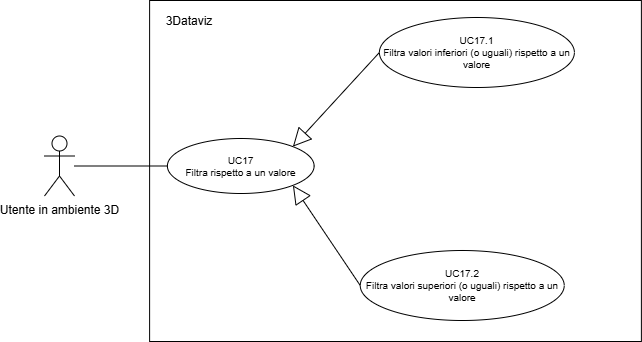
\includegraphics[scale=0.7]{template/images/UC17.png}
    \caption{\nameref*{UC:\arabic{UC}}}
\end{figure}
\UCdsc
{ % ATTORE
    \begin{itemize}
        \item Utente in ambiente 3D.
    \end{itemize}
}
{ % DESCRIZIONE
    \begin{itemize}
        \item Questo filtro consente all'utente di visualizzare solo le barre che hanno un valore superiore, inferiore o uguale rispetto a un valore scelto dall’utente. 
    \end{itemize}
}
{ % PRECONDIZIONI
    \begin{itemize}
        \item Il grafico è visibile.
    \end{itemize}
}
{ % POSTCONDIZIONI
    \begin{itemize}
        \item È stato applicato il filtro per visualizzare solo le barre con un valore superiore, inferiore o uguale rispetto a un valore scelto dall’utente.
    \end{itemize}
}
{ % SCENARIO PRIMARIO
    \begin{itemize}
        \item L’utente seleziona un valore;
        \item Il sistema aggiorna la visualizzazione del grafico, evidenziando le barre che rientrano nella condizione scelta.
    \end{itemize}
  % GENERALIZZAZIONI
        \item \textbf{Generalizzazioni:} \begin{itemize}
            \item UC17.1 - Filtra valori inferiori (o uguali) rispetto a un valore;
            \item UC17.2 - Filtra valori superiori (o uguali) rispetto a un valore.
        \end{itemize}
    
}


\SubUseCase{Filtra valori inferiori (o uguali) rispetto a un valore}
\begin{figure}[H]\centering
    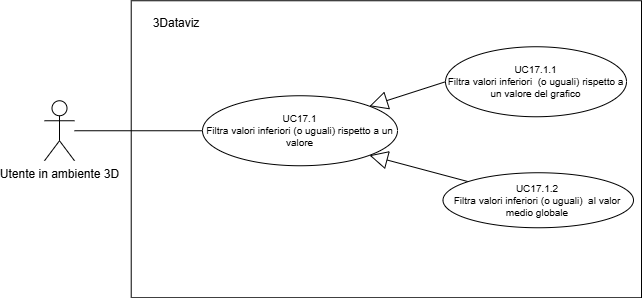
\includegraphics[scale=0.7]{template/images/UC17.1.png}
    \caption{\nameref*{UC:\arabic{UC}.\arabic{SUC}}}
\end{figure}
\UCdsc
{ % ATTORE
    \begin{itemize}
        \item Utente in ambiente 3D.
    \end{itemize}
}
{ % DESCRIZIONE
    \begin{itemize}
        \item L'utente decide di evidenziare i valori inferiori (o uguali) rispetto a un valore, rendendo visibili le barre corrispondenti a questo criterio.
    \end{itemize}
}
{ % PRECONDIZIONI
    \begin{itemize}
        \item Il grafico è visibile;
        \item L'utente ha scelto il filtro rispetto a un valore.
    \end{itemize}
}
{ % POSTCONDIZIONI
    \begin{itemize}
        \item Le barre con valori che non soddisfano il criterio di essere inferiori (o uguali) al valore scelto diventano più trasparenti.
    \end{itemize}
}
{ % SCENARIO PRIMARIO
    \begin{itemize}
        \item L'utente seleziona l'opzione per visualizzare le barre inferiori (o uguali).
    \end{itemize}
    % GENERALIZZAZIONI
    \item \textbf{Generalizzazioni:} \begin{itemize}
        \item UC17.1.1 - Filtra valori inferiori (o uguali) rispetto a un valore del grafico;
        \item UC17.2.2 - Filtra valori inferiori (o uguali) rispetto al valor medio globale.
    \end{itemize}
}



\SubSubUseCase{Filtra valori inferiori (o uguali) rispetto a un valore del grafico}
\UCdsc
{ % ATTORE
    \begin{itemize}
        \item Utente in ambiente 3D.
    \end{itemize}
}
{ % DESCRIZIONE
    \begin{itemize}
        \item L'utente decide di evidenziare i valori inferiori (o uguali) rispetto a un valore del grafico, rendendo visibili le barre corrispondenti a questo criterio.
    \end{itemize}
}
{ % PRECONDIZIONI
    \begin{itemize}
        \item Il grafico è visibile;
        \item L'utente ha scelto il filtro di valori inferiori (o uguali).
    \end{itemize}
}
{ % POSTCONDIZIONI
    \begin{itemize}
        \item Le barre con valori che non soddisfano il criterio di essere inferiori (o uguali) rispetto a un valore del grafico selezionato diventano più trasparenti.
    \end{itemize}
}
{ % SCENARIO PRIMARIO
    \begin{itemize}
        \item L'utente seleziona l'opzione per visualizzare le barre inferiori (o uguali) rispetto a un valore del grafico.
    \end{itemize}
}


\SubSubUseCase{Filtra valori inferiori (o uguali) rispetto al valor medio globale}
\UCdsc
{ % ATTORE
    \begin{itemize}
        \item Utente in ambiente 3D.
    \end{itemize}
}
{ % DESCRIZIONE
    \begin{itemize}
        \item L'utente decide di evidenziare i valori inferiori (o uguali) rispetto al valor medio globale, rendendo visibili le barre corrispondenti a questo criterio.
    \end{itemize}
}
{ % PRECONDIZIONI
    \begin{itemize}
        \item Il grafico è visibile;
        \item L'utente ha scelto il filtro di valori inferiori (o uguali).
    \end{itemize}
}
{ % POSTCONDIZIONI
    \begin{itemize}
        \item Le barre con valori che non soddisfano il criterio di essere inferiori (o uguali) rispetto al valor medio globale diventano più trasparenti.
    \end{itemize}
}
{ % SCENARIO PRIMARIO
    \begin{itemize}
        \item L'utente seleziona l'opzione per visualizzare le barre inferiori (o uguali) rispetto al valor medio globale.
    \end{itemize}
}




\SubUseCase{Filtra valori superiori (o uguali) rispetto a un valore}
\begin{figure}[H]\centering
    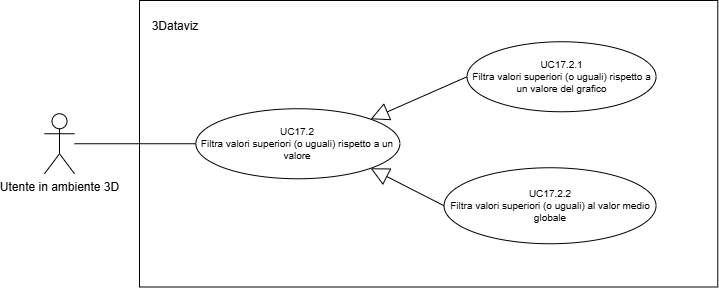
\includegraphics[scale=0.6]{template/images/UC17.2.png}
    \caption{\nameref*{UC:\arabic{UC}.\arabic{SUC}}}
\end{figure}
\UCdsc
{ % ATTORE
    \begin{itemize}
        \item Utente in ambiente 3D.
    \end{itemize}
}
{ % DESCRIZIONE
    \begin{itemize}
        \item L'utente decide di evidenziare i valori superiori (o uguali) rispetto a un valore, rendendo visibili le barre corrispondenti a questo criterio.
    \end{itemize}
}
{ % PRECONDIZIONI
    \begin{itemize}
        \item Il grafico è visibile;
        \item L'utente ha scelto il filtro rispetto a un valore.
    \end{itemize}
}
{ % POSTCONDIZIONI
    \begin{itemize}
        \item Le barre dei valori che non rientrano in questa condizione diventano più trasparenti.
    \end{itemize}
}
{ % SCENARIO PRIMARIO
    \begin{itemize}
        \item L'utente seleziona l'opzione per visualizzare le barre superiori (o uguali).
    \end{itemize}
    % GENERALIZZAZIONI
    \item \textbf{Generalizzazioni:} \begin{itemize}
        \item UC17.1.1 - Filtra valori superiori (o uguali) rispetto a un valore del grafico;
        \item UC17.2.2 - Filtra valori superiori (o uguali) rispetto al valor medio globale.
    \end{itemize}
}


\SubSubUseCase{Filtra valori superiori (o uguali) rispetto a un valore del grafico}
\UCdsc
{ % ATTORE
    \begin{itemize}
        \item Utente in ambiente 3D.
    \end{itemize}
}
{ % DESCRIZIONE
    \begin{itemize}
        \item L'utente decide di evidenziare i valori superiori (o uguali) rispetto a un valore del grafico, rendendo visibili le barre corrispondenti a questo criterio.
    \end{itemize}
}
{ % PRECONDIZIONI
    \begin{itemize}
        \item Il grafico è visibile;
        \item L'utente ha scelto il filtro di valori superiori (o uguali).
    \end{itemize}
}
{ % POSTCONDIZIONI
    \begin{itemize}
        \item Le barre con valori che non soddisfano il criterio di essere superiori (o uguali) rispetto a un valore del grafico selezionato diventano più trasparenti.
    \end{itemize}
}
{ % SCENARIO PRIMARIO
    \begin{itemize}
        \item L'utente seleziona l'opzione per visualizzare le barre superiori (o uguali) rispetto a un valore del grafico.
    \end{itemize}
}


\SubSubUseCase{Filtra valori superiori (o uguali) rispetto al valor medio globale}
\UCdsc
{ % ATTORE
    \begin{itemize}
        \item Utente in ambiente 3D.
    \end{itemize}
}
{ % DESCRIZIONE
    \begin{itemize}
        \item L'utente decide di evidenziare i valori superiori (o uguali) rispetto al valor medio globale, rendendo visibili le barre corrispondenti a questo criterio.
    \end{itemize}
}
{ % PRECONDIZIONI
    \begin{itemize}
        \item Il grafico è visibile;
        \item L'utente ha scelto il filtro di valori superiori (o uguali).
    \end{itemize}
}
{ % POSTCONDIZIONI
    \begin{itemize}
        \item Le barre con valori che non soddisfano il criterio di essere superiori (o uguali) rispetto al valor medio globale diventano più trasparenti.
    \end{itemize}
}
{ % SCENARIO PRIMARIO
    \begin{itemize}
        \item L'utente seleziona l'opzione per visualizzare le barre superiori (o uguali) rispetto al valor medio globale.
    \end{itemize}
}


\UseCase{Reset dei filtri}
\begin{figure}[H]\centering
    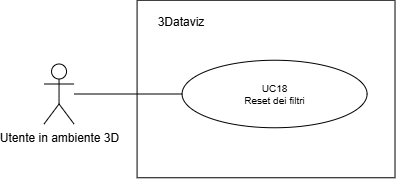
\includegraphics[scale=0.7]{template/images/UC18.png}
    \caption{\nameref*{UC:\arabic{UC}}}
\end{figure}
\UCdsc
{ % ATTORE
    \begin{itemize}
        \item Utente in ambiente 3D.
    \end{itemize}
}
{ % DESCRIZIONE
    \begin{itemize}
        \item L'utente può reimpostare tutti i filtri applicati al grafico, riportando la visualizzazione allo stato iniziale, con tutte le barre visibili senza alcun filtro attivo.
    \end{itemize}
}
{ % PRECONDIZIONI
    \begin{itemize}
        \item Il grafico è visibile;
        \item Almeno un filtro è stato applicato alla visualizzazione.
    \end{itemize}
}
{ % POSTCONDIZIONI
    \begin{itemize}
        \item Tutti i filtri applicati sono rimossi;
        \item Il grafico ritorna al suo stato iniziale.
    \end{itemize}
}
{ % SCENARIO PRIMARIO
    \begin{itemize}
        \item L'utente seleziona l'opzione di reset dei filtri;
        \item Il sistema rimuove tutti i filtri applicati.
    \end{itemize}
}


\UseCase{Visualizza piano del valor medio}
\begin{figure}[H]\centering
    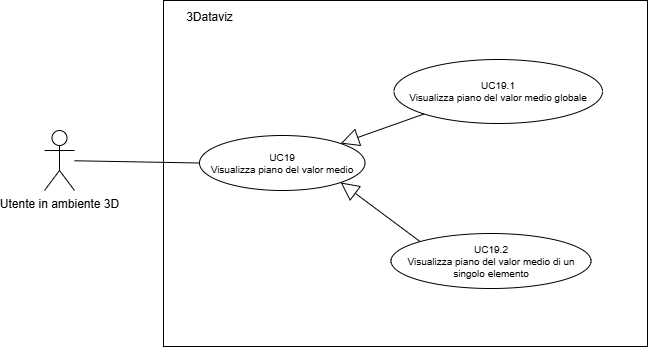
\includegraphics[scale=0.7]{template/images/UC19.png}
    \caption{\nameref*{UC:\arabic{UC}}}
\end{figure}
\UCdsc
{ % ATTORE
    \begin{itemize}
        \item Utente in ambiente 3D.
    \end{itemize}
}
{ % DESCRIZIONE
    \begin{itemize}
        \item Visualizzazione di un piano parallelo alla base nel grafico 3D per evidenziare il valor medio.
    \end{itemize}
}
{ % PRECONDIZIONI
    \begin{itemize}
        \item Il grafico è visibile.
    \end{itemize}
}
{ % POSTCONDIZIONI
    \begin{itemize}
        \item Il piano che rappresenta il valor medio è visibile.
    \end{itemize}
}
{ % SCENARIO PRIMARIO
    \begin{itemize}
        \item L'utente seleziona l'opzione per visualizzare il valor medio.
    \end{itemize}
}


\SubUseCase{Visualizza piano del valor medio globale}
\UCdsc
{ % ATTORE
    \begin{itemize}
        \item Utente in ambiente 3D.
    \end{itemize}
}
{ % DESCRIZIONE
    \begin{itemize}
        \item Viene visualizzato un piano parallelo alla base che rappresenta la media globale dei valori del dataset.
    \end{itemize}
}
{ % PRECONDIZIONI
    \begin{itemize}
        \item Il grafico è visibile.
    \end{itemize}
}
{ % POSTCONDIZIONI
    \begin{itemize}
        \item Il piano che rappresenta il valor medio globale è visibile.
    \end{itemize}
}
{ % SCENARIO PRIMARIO
    \begin{itemize}
        \item L'utente seleziona l'opzione per visualizzare il valor medio;
        \item L'utente seleziona l'opzione del valor medio globale.
    \end{itemize}
}

\SubUseCase{Visualizza piano della media dei valori relativi a un etichetta}
\UCdsc
{ % ATTORE
    \begin{itemize}
        \item Utente in ambiente 3D.
    \end{itemize}
}
{ % DESCRIZIONE
    \begin{itemize}
        \item Viene visualizzato un piano parallelo alla base che rappresenta la media dei valori relativi a una determinata etichetta di un asse.
    \end{itemize}
}
{ % PRECONDIZIONI
    \begin{itemize}
        \item Il grafico è visibile.
    \end{itemize}
}
{ % POSTCONDIZIONI
    \begin{itemize}
        \item Il piano che rappresenta il valor medio di un singolo elemento è visibile.
    \end{itemize}
}
{ % SCENARIO PRIMARIO
    \begin{itemize}
        \item L'utente seleziona l'opzione per visualizzare il valor medio;
        \item L'utente seleziona l'etichetta su quale genererare il valor medio.
    \end{itemize}
}









\pagebreak

\newcounter{RF1}
\newcounter{RF2}
\newcounter{RF3}
\newcounter{RV1}
\newcounter{RV2}
\newcounter{RV3}
\newcounter{RP1}
\newcounter{RP2}
\newcounter{RP3}
\newcounter{RQ1}
\newcounter{RQ2}
\newcounter{RQ3}

\newcounter{RF}
\newcounter{RV}
\newcounter{RP}
\newcounter{RQ}

\newcounter{M}
\newcounter{D}
\newcounter{O}

\newcommand{\RFM}{
    \stepcounter{M}
    \stepcounter{RF}
    \stepcounter{RF1}
    RF\arabic{RF}
}
\newcommand{\RFD}{
    \stepcounter{D}
    \stepcounter{RF}
    \stepcounter{RF2}
    RF\arabic{RF}
}
\newcommand{\RFO}{
    \stepcounter{O}
    \stepcounter{RF}
    \stepcounter{RF3}
    RF\arabic{RF}
}
\newcommand{\RVM}{
    \stepcounter{M}
    \stepcounter{RV}
    \stepcounter{RV1}
    RV\arabic{RV}
}
\newcommand{\RVD}{
    \stepcounter{D}
    \stepcounter{RV}
    \stepcounter{RV2}
    RV\arabic{RV}
}
\newcommand{\RVO}{
    \stepcounter{O}
    \stepcounter{RV}
    \stepcounter{RV3}
    RV\arabic{RV}
}
\newcommand{\RPM}{
    \stepcounter{M}
    \stepcounter{RP}
    \stepcounter{RP1}
    RP\arabic{RP}
}
\newcommand{\RPD}{
    \stepcounter{D}
    \stepcounter{RP}
    \stepcounter{RP2}
    RP\arabic{RP}
}
\newcommand{\RPO}{
    \stepcounter{O}
    \stepcounter{RP}
    \stepcounter{RP3}
    RP\arabic{RP}
}
\newcommand{\RQM}{
    \stepcounter{M}
    \stepcounter{RQ}
    \stepcounter{RQ1}
    RQ\arabic{RQ}
}
\newcommand{\RQD}{
    \stepcounter{D}
    \stepcounter{RQ}
    \stepcounter{RQ2}
    RQ\arabic{RQ}
}
\newcommand{\RQO}{
    \stepcounter{O}
    \stepcounter{RQ}
    \stepcounter{RQ3}
    RQ\arabic{RQ}
}


\newcommand{\requirementsTable}[1]{

\renewcommand{\arraystretch}{1.5}
\rowcolors{2}{pari}{dispari}
\begin{longtable}{ %0.87
		>{\centering}M{0.15\textwidth} 
		>{\centering}M{0.5\textwidth}
		>{\centering}M{0.20\textwidth}
		>{\centering\arraybackslash}M{0.15\textwidth} 
		 }
	\rowcolorhead
	\headertitle{Requisito} &
	\centering \headertitle{Descrizione} &	
	\headertitle{Classificazione} &
	\headertitle{Fonte}
	\endfirsthead	
	\endhead
	
	#1

\end{longtable}
\vspace{2em}

}

\newcommand{\SrcToReqTable}[1]{

\renewcommand{\arraystretch}{1.5}
\rowcolors{2}{pari}{dispari}
\begin{longtable}{ %0.87
		>{\centering}M{0.5\textwidth} 
		>{\centering\arraybackslash}M{0.20\textwidth} 
		 }
	\rowcolorhead
	\headertitle{Fonte} &
	\centering\headertitle{Requisito}
	\endfirsthead	
	\endhead
	
	#1

\end{longtable}
\vspace{2em}

}

\newcommand{\ReqToUCTable}[1]{

\renewcommand{\arraystretch}{1.5}
\rowcolors{2}{pari}{dispari}
\begin{longtable}{ %0.87
		>{\centering}M{0.5\textwidth} 
		>{\centering\arraybackslash}M{0.20\textwidth} 
		 }
	\rowcolorhead
	\headertitle{Requisito} &
	\centering\headertitle{Fonte}
	\endfirsthead	
	\endhead
	
	#1

\end{longtable}
\vspace{2em}

}

\newcommand{\requirementsSummaryTable}[1]{

\renewcommand{\arraystretch}{1.5}
\rowcolors{2}{pari}{dispari}
\begin{longtable}{ %0.87
		>{\centering}M{0.3\textwidth} 
		>{\centering}M{0.15\textwidth}
		>{\centering}M{0.15\textwidth}
		>{\centering}M{0.15\textwidth}
		>{\centering\arraybackslash}M{0.15\textwidth} 
		 }
	\rowcolorhead
	\headertitle{Tipologia} &
	\centering \headertitle{Obbligatorio} &	
	\headertitle{Desiderabile} &
	\headertitle{Opzionale} &
	\headertitle{Totale}
	\endfirsthead	
	\endhead
	
	#1

\end{longtable}
\vspace{2em}

}

\section{Requisiti}
\subsection{Introduzione}
Sono stati definiti dei requisiti codificati in base all’ambito di competenza e ad un numero seriale per
tenerne meglio traccia. Nelle tabelle sottostanti sono forniti descrizione e classificazione di ciascun
requisito. 
Per la codifica dei requisiti si faccia riferimento alle \textit{Norme di progetto}.
\subsection{Requisiti funzionali}
\requirementsTable{
    % VISUALIZZAZIONE DATASET
    \RFM & L’utente deve poter visualizzare i dataset  & Obbligatorio & UC1 \tabularnewline
    \RFM & L’utente deve poter visualizzare le informazioni primarie dei dataset  & Obbligatorio & UC1.1\par UC1.1.1\par UC1.1.2 \tabularnewline
    \RFM & L’utente deve poter visualizzare i dettagli dei dataset  & Obbligatorio  & UC2\par UC2.1 \tabularnewline

    % CARICAMENTO DATASET
    \RFM & L’utente deve poter caricare il dataset &  Obbligatorio &UC3\tabularnewline
    \RFM & L’utente deve ricevere un errore se il caricamento di un dataset fallisce  & Obbligatorio& UC4\tabularnewline

    % VISUALIZZAZIONE DEI DATI IN TABELLA
    \RFM & L’utente deve poter visualizzare i dati del dataset selezionato in forma tabellare & Obbligatorio   & UC5\tabularnewline
    \RFM & L’utente deve poter visualizzare le intestazioni della tabella  & Obbligatorio  & UC5.1 \tabularnewline
    \RFM & L’utente deve poter visualizzare il valore del dato in una cella della tabella  & Obbligatorio  & UC5.2 \tabularnewline
    
    % VISUALIZZAZIONE DEI DATI SUL GRAFICO
    \RFM & L’utente deve poter visualizzare i dati del dataset selezionato in forma di grafico tridimensionale a barre verticali  & Obbligatorio  &  UC6\tabularnewline
    \RFM & L’utente deve poter visualizzare gli assi del grafico tridimensionale  & Obbligatorio   &  UC6.1\tabularnewline
    \RFM & L’utente deve poter visualizzare l'asse X del grafico tridimensionale   & Obbligatorio  & UC6.1.1 \tabularnewline
    \RFM & L’utente deve poter visualizzare l'asse Y del grafico tridimensionale   & Obbligatorio  & UC6.1.2 \tabularnewline
    \RFM & L’utente deve poter visualizzare l'asse Z del grafico tridimensionale   & Obbligatorio  & UC6.1.3 \tabularnewline

    
    % TELECAMERA
    \RFM & L’utente deve poter muovere la telecamera orizzontalmente & Obbligatorio  &  UC7\tabularnewline
    \RFM & L’utente deve poter muovere la telecamera verticalmente  & Obbligatorio &  UC8\tabularnewline
    
    % TELECAMERA
    \RFM & L’utente deve poter ruotare il grafico attorno all'asse X   & Obbligatorio & UC9\tabularnewline
    \RFM & L’utente deve poter ruotare il grafico attorno all'asse Y  & Obbligatorio  & UC10\tabularnewline
    \RFM & L’utente deve poter ruotare il grafico attorno all'asse Z   & Obbligatorio & UC11\tabularnewline
    
    %ZOOM
    \RFM & L’utente deve poter eseguire un’azione di zoom indipendentemente dalla posizione della telecamera & Obbligatorio & UC12\tabularnewline

    %RIPOSIONNAMENTO
    \RFM & L’utente deve poter riposizionare la telecamera alla sua posizione iniziale  & Obbligatorio  & UC13\tabularnewline

    %VISUALIZZAZIONE PRIMO PIANO
    \RFM & L’utente deve poter visualizzare una singola barra del grafico in primo piano  & Obbligatorio & UC14\tabularnewline

    %VISUALIZZAZIONE DETTAGLI
    \RFM & L’utente deve poter visualizzare i dettagli di una barra del grafico  & Obbligatorio & UC15\par UC15.1\par UC15.2\tabularnewline

    %FILTRI
    \RFM & L’utente deve poter filtrare un numero N dei valori più alti & Obbligatorio & UC16\par UC16.1\tabularnewline
    \RFM & L’utente deve poter filtrare un numero N dei valori più bassi & Obbligatorio & UC16\par UC16.2\tabularnewline
    \RFM & L’utente deve poter inserire un numero per effettuare un filtraggio & Obbligatorio & UC16\par UC16.3\tabularnewline
    \RFM & L’utente deve poter filtrare i valori inferiori o uguali rispetto a un valore del grafico & Obbligatorio & UC17\par UC17.1\par UC17.1.1\tabularnewline
    \RFM & L’utente deve poter filtrare i valori inferiori o uguali rispetto al valor medio globale & Obbligatorio & UC17\par UC17.1\par UC17.1.2\tabularnewline
    \RFM & L’utente deve poter filtrare i valori superiori o uguali rispetto a un valore del grafico & Obbligatorio & UC17\par UC17.2\par UC17.2.1\tabularnewline
    \RFM & L’utente deve poter filtrare i valori superiori o uguali rispetto al valor medio globale & Obbligatorio & UC17\par UC17.2\par UC17.2.2\tabularnewline

    %RESET
    \RFM & L’utente deve poter ripristinare lo stato del grafico
    rispetto ai precedenti filtri applicati   & Obbligatorio & UC18\tabularnewline

    %VALOR MEDIO
    \RFM & L’utente deve poter visualizzare un piano parallelo alla base che rappresenti il valor medio globale & Obbligatorio & UC19\par UC19.1\tabularnewline
    \RFD & L’utente deve poter visualizzare un piano parallelo alla base che rappresenti la media dei valori relativi a un etichetta & Desiderabile & UC19\par UC19.2\tabularnewline

    %COLORE
    \RFO & Le barre del grafico 3D devono avere una colorazione appropriata che renda i relativi valori facilmente e velocemente comprensibili  & Opzionale & VE 2024-12-19 \tabularnewline

    }

   
\subsection{Requisiti qualitativi}
    
\requirementsTable{
    \RQM & Il software deve essere sviluppato seguendo le metriche e il modello di qualità descritti nel documento \textit{Norme di progetto}  & Obbligatorio  & Decisione interna \tabularnewline
    \RQM & Il software deve essere sviluppato pubblicando il codice sorgente nel repository Github dedicato  & Obbligatorio  & Decisione interna \tabularnewline
    \RQM & Il software deve essere sviluppato in modo tale da supportare grandi volumi di dati   & Obbligatorio & Capitolato \tabularnewline
    \RQM & L'architettura del software deve permettere, con agilità, di aggiungere nuove funzionalità e possibilità di iterazione con il grafico   & Obbligatorio  & Capitolato \tabularnewline
    \RQM & La suite di test deve essere robusta per garantire quanto specificato nel RQ4  & Obbligatorio  & Capitolato \tabularnewline
    \RQD & Il software deve essere testato attraverso test di tipo e2e  & Desiderabile  & Capitolato \tabularnewline  
}
 \pagebreak
\subsection{Requisiti di vincolo}
\requirementsTable{
    \RVM & Il software deve essere sviluppato utilizzando Typescript come linguaggio di programmazione primario  & Obbligatorio  & Decisione interna \tabularnewline
    \RVM & Il software deve essere sviluppato utilizzando la libreria React per la creazione di un'interfaccia visiva semplice  & Obbligatorio  & Decisione interna \tabularnewline
    \RVM & Il software deve essere sviluppato utilizzando la libreria Three.js   & Obbligatorio & Decisione interna \tabularnewline
    \RVM & Il software deve essere compatibile dalla versione 131 del browser Chrome  & Obbligatorio & Decisione interna \tabularnewline
    \RVM & Il software deve essere compatibile dalla versione 133 del browser Firefox  & Obbligatorio & Decisione interna \tabularnewline
    \RVM & Il software deve essere compatibile dalla versione 115 del browser Opera  & Obbligatorio & Decisione interna \tabularnewline
    \RVM & Il software deve essere compatibile dalla versione 131 del browser Microsoft Edge  & Obbligatorio & Decisione interna \tabularnewline
    }
\newpage

\subsection{Requisiti prestazionali}
\requirementsTable{
    \RPM & Il software quando carica un dataset di dimensioni minori o uguali a 100000 non deve avere un tempo di caricamento superiore a 2 secondi  & Obbligatorio & Decisione interna \tabularnewline
    \RPM & Il software quando carica un dataset di dimensioni minori o uguali a 500000 non deve avere un tempo di caricamento superiore a 5 secondi  & Obbligatorio & Decisione interna \tabularnewline
    \RPM & Il software quando carica un dataset di dimensioni minori o uguali a 1000000 non deve avere un tempo di caricamento superiore a 8 secondi  & Obbligatorio & Decisione interna \tabularnewline
    \RPD & Il software quando carica un dataset di dimensioni maggiori a 1000000 non deve avere un tempo di caricamento superiore a 15 secondi  & Desiderabile & Decisione interna \tabularnewline
    \RPM & Il software non deve avere un tempo di risposta superiore a 5 secondi & Obbligatorio & Decisione interna \tabularnewline
}


\subsection{Tracciamento requisiti}

\subsubsection{Fonte - Requisiti}
\SrcToReqTable{
    Capitolato & RQ3\par RQ4\par RQ5\par RQ6\par RV8 \tabularnewline
    Decisione interna & RQ1\par
                        RQ2\par 
                        RV1\par 
                        RV2\par 
                        RV3\par 
                        RV4\par
                        RV5\par
                        RV6\par
                        RV7\par
                        RP1\par
                        RP2\par
                        RP3\par
                        RP4\par
                        RP5\par
                        \tabularnewline
    UC1    & RF1 \tabularnewline
    UC1.1    & RF2 \tabularnewline
    UC1.1.1    & RF2 \tabularnewline
    UC1.1.2    & RF2 \tabularnewline
    UC2    & RF3 \tabularnewline
    UC2.1    & RF3 \tabularnewline
    UC3    & RF4 \tabularnewline
    UC4   & RF5 \tabularnewline
    UC5    & RF6 \tabularnewline
    UC5.1    & RF7 \tabularnewline
    UC5.2    & RF8 \tabularnewline
    UC6    & RF9 \tabularnewline
    UC6.1    & RF10 \tabularnewline
    UC6.1.1    & RF11 \tabularnewline
    UC6.1.2    & RF12 \tabularnewline
    UC6.1.3    & RF13 \tabularnewline
    UC7    & RF14 \tabularnewline
    UC8   & RF15 \tabularnewline
    UC9    & RF16 \tabularnewline
    UC10    & RF17 \tabularnewline
    UC11   & RF18 \tabularnewline
    UC12    & RF19 \tabularnewline
    UC13    & RF20 \tabularnewline
    UC14   & RF21 \tabularnewline
    UC15    & RF22 \tabularnewline
    UC15.1    & R22 \tabularnewline
    UC15.2    & RF22 \tabularnewline
    UC16    & RF23\par RF24\par RF25 \tabularnewline
    UC16.1    & RF23 \tabularnewline
    UC16.2    & RF24 \tabularnewline
    UC16.3    & RF25 \tabularnewline
    UC17    & RF26\par RF27\par RF28\par RF29 \tabularnewline
    UC17.1    & RF26\par RF27 \tabularnewline
    UC17.1.1    & RF26 \tabularnewline
    UC17.1.2    & RF27 \tabularnewline
    UC17.2    & RF28\par RF29 \tabularnewline
    UC17.2.1    & RF28 \tabularnewline
    UC17.2.2    & RF29 \tabularnewline
    UC18   & RF30 \tabularnewline
    UC19   & RF31\par RF32 \tabularnewline
    UC19.1    & RF31 \tabularnewline
    UC19.2    & RF32 \tabularnewline
    VE 2024-12-19  & RF33 \tabularnewline

    }

\subsubsection{Requisiti - Fonti}
\ReqToUCTable{

    RF1 & UC1 \tabularnewline
    RF2 & UC1.1\par UC1.1.1\par UC1.1.2\tabularnewline
    RF3 & UC2\par UC2.1 \tabularnewline
    RF4 & UC3 \tabularnewline
    RF5 & UC4 \tabularnewline
    RF6 & UC5 \tabularnewline
    RF7 & UC5.1 \tabularnewline
    RF8 & UC5.2 \tabularnewline
    RF9 & UC6 \tabularnewline
    RF10 & UC6.1 \tabularnewline
    RF11 & UC6.1.1 \tabularnewline
    RF12 & UC6.1.2 \tabularnewline
    RF13 & UC6.1.3 \tabularnewline
    RF14 & UC7 \tabularnewline
    RF15 & UC8 \tabularnewline
    RF16 & UC9 \tabularnewline
    RF17 & UC10 \tabularnewline
    RF18 & UC11\tabularnewline
    RF19 & UC12 \tabularnewline
    RF20 & UC13 \tabularnewline
    RF21 & UC14 \tabularnewline
    RF22 & UC15\par UC15.1\par UC15.2 \tabularnewline
    RF23 & UC16\par UC16.1 \tabularnewline
    RF24 & UC16\par UC16.2 \tabularnewline
    RF25 & UC16\par UC16.3 \tabularnewline
    RF26 & UC17\par UC17.1\par UC17.1.1 \tabularnewline
    RF27 & UC17\par UC17.1\par UC17.1.2 \tabularnewline
    RF28 & UC17\par UC17.2\par UC17.2.1 \tabularnewline
    RF29 & UC17\par UC17.2\par UC17.2.2 \tabularnewline
    RF30 & UC18 \tabularnewline
    RF31 & UC19\par UC19.1 \tabularnewline
    RF32 & UC19\par UC19.2 \tabularnewline
    RF33 & VE 2024-12-19  \tabularnewline

    RQ1 & Decisione interna\tabularnewline
    RQ2 & Decisione interna\tabularnewline
    RQ3 & Capitolato\tabularnewline
    RQ4 & Capitolato\tabularnewline
    RQ5 & Capitolato\tabularnewline
    RQ6 & Capitolato\tabularnewline

    RV1 & Decisione interna\tabularnewline
    RV2 & Decisione interna\tabularnewline
    RV3 & Decisione interna\tabularnewline
    RV4 & Decisione interna\tabularnewline
    RV5 & Decisione interna\tabularnewline
    RV6 & Decisione interna\tabularnewline
    RV7 & Decisione interna\tabularnewline
    RV7 & Capitolato\tabularnewline

    RP1 & Decisione interna\tabularnewline
    RP2 & Decisione interna\tabularnewline
    RP3 & Decisione interna\tabularnewline
    RP4 & Decisione interna\tabularnewline
    RP5 & Decisione interna\tabularnewline

}

\newcounter{T}

\addtocounter{T}{\value{M}}
\addtocounter{T}{\value{D}}
\addtocounter{T}{\value{O}}



\subsubsection{Riepilogo requisiti}
\requirementsSummaryTable{
    Funzionale & \arabic{RF1} & \arabic{RF2} & \arabic{RF3} & \arabic{RF} \tabularnewline
    Di qualità & \arabic{RQ1} & \arabic{RQ2} & \arabic{RQ3} & \arabic{RQ} \tabularnewline
    Di vincolo & \arabic{RV1} & \arabic{RV2} & \arabic{RV3} & \arabic{RV} \tabularnewline
    Prestazionali & \arabic{RP1} & \arabic{RP2} & \arabic{RP3} & \arabic{RP} \tabularnewline
    \bottomrule
    \textbf{Totale requisiti} & \arabic{M} & \arabic{D} & \arabic{O} & \arabic{T}
    
}


\pagebreak

% insert here other content (\include)


\end{document}


